% ---
% Capitulo de METODOLOGIA
% ---
\chapter{Metodologia}\label{cap:metodologia}
Trata-se de um estudo descritivo e exploratório sobre e-learning, gameficação e TEA. Para isso, a obtenção do conhecimento foi dada por material bibliográfico, o qual foi adquirido através de livros e artigos científicos, assim como, por entrevistas com alguns profissionais do ramo da psicologia; da terapia ocupacional e da fonoaudiologia, todos atuantes no tratamento de crianças com TEA.

A apresentação dos resultados é dada de forma descritiva utilizando alguns artefatos da metodologia RUP (Rational Unified Process) para documentar a especificação do sistema e validar o produto gerado por este trabalho.

Na seção \ref{rup} apresentamos o processo RUP e a configuração feita em seus processos para adequar o desenvolvimento deste trabalho.

\section{Rup - Rational Unified Process}\label{rup}
O RUP é um processo de engenharia de software proprietário da IBM\footnote{Acesse: www.ibm.com} que fornece uma linha de base para o desenvolvimento de um software, utilizando uma abordagem disciplinada para designar tarefas e responsabilidades dentro do projeto. Tem como objetivo, atender às necessidades dos clientes com um software de alta qualidade sem extrapolar o cronograma e nem o orçamento designado. O RUP é configurável e pode ser adaptado a projetos de software e equipes desenvolvimento de todos os tamanhos. Atualmente existe uma versão\footnote{Acesse: http://www.funpar.ufpr.br:8080/rup/process/ovu\_proc.htm} traduzida para o português e mantida pela Fundação da Universidade Federal do Paraná, contendo toda a linha de base do processo RUP.
%(http://www.funpar.ufpr.br:8080/rup/process/ovu_proc.htm).
%https://www.ibm.com/developerworks/rational/library/content/03July/1000/1251/1251_bestpractices_TP026B.pdf

\begin{figure}[H]
	\centering
	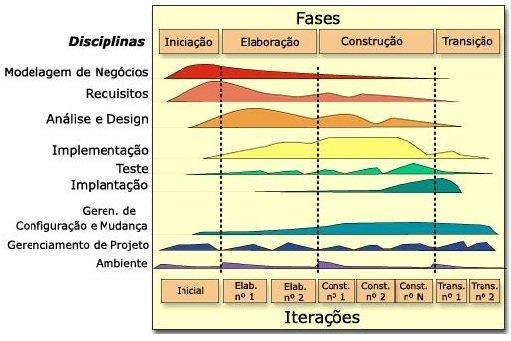
\includegraphics[scale=0.6]{img/fasesdisciplinaRUP.jpg}
	\caption{Modelo RUP}
	\label{modelorup}
	Fonte:Funpar UFPR
\end{figure}

O Modelo RUP completo pode ser explicado de forma bidimensional, tendo dois eixos: o do tempo e o do conteúdo. No eixo do tempo existem 4 fases, as quais são subdivididas em iterações, e são concluídas em um marco. No eixo do conteúdo existem 9 disciplinas de software, cada qual contendo seus fluxos de trabalho com as atividades desemplenhadas por cada papel para entregar os artefatos.
%http://www.funpar.ufpr.br:8080/rup/process/itrwkfls/iwf_iwfs.htm

\begin{figure}[H]
	\centering
	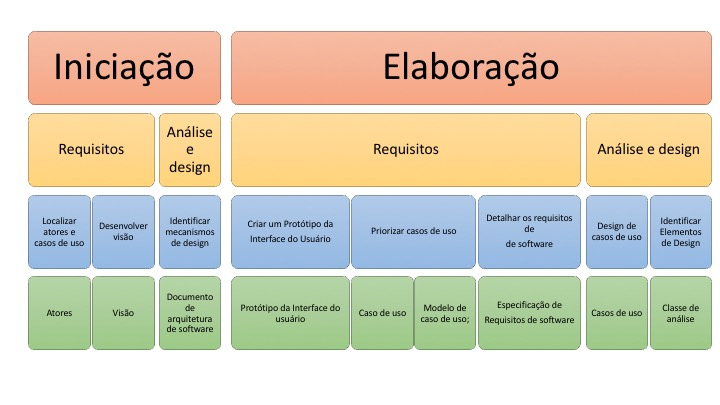
\includegraphics[scale=0.6]{img/eaprup.jpeg}
	\caption{EAP}
	\label{eaprup}
	Fonte:Autor, 2018
\end{figure}


Na fase de iniciação, tivemos a realização primeiramente da disciplinas de requisito onde teve-se como atividades localizar atores e casos de uso dessa forma obtivemos como artefatos os atores que usaram o sistema e o desenvolvimento da visão onde foi possível definir como os envolvido enxergaram o sistema e sobre as necessidades que ele precisa sanar com a utilização.

Em seguida, houve a realização da disciplina de análise de requisitos da ainda da fase iniciação, no qual foram realizadas as atividade de identificação dos mecanismos de design, tendo como artefato gerado o documento de arquitetura de software onde foi houve o planejamento de como seria a arquitetura de funcionamento do aplicativo.

Na fase de elaboração, tivemos a realização primeiramente da disciplina de requisitos, onde houve como  atividade a criação de um protótipo da interface de usuário, na qual gerou como artefato o protótipo de interface do usuário e a atividade priorizar caso de uso onde obtivemos como artefato os casos de uso do sistema a ser implementado e a atividade de detalhar os requisitos de software na qual tivemos como artefato a especificação dos requisitos funcionais do aplicativo.

Ainda na fase de elaboração, houve a realização da disciplina de análise e design, na qual foram realizadas  a atividade de  design de caso de uso, onde obtivemos como artefato a validação e correção dos casos de uso gerados anteriormente e por fim a atividade de identificar elementos de design, na qual obtivemos como resultados as classes do sistema, como o levantamento do diagrama de classes.

\section{Considerações Finais}
Este capítulo apresentou a metodologia usada durante o processo de desenvolvimento deste trabalho. Foi apresentado a metodologia RUP, que é o processo de engenharia de software usado para a geração dos resultados deste trabalho. A seguir será apresentados os trabalhos que tem o mesmo teor desta pesquisa, são apresentados cinco artigos e cinco aplicativos disponíveis na \textit{Google Play Store}, ainda no capítulo dos trabalhos relacionados são apresentados os fatores que diferem este trabalho dos demais citados. No capítulo seguinte são apresentados os resultados obtidos durante a pesquisa.